%%%%%%%%%%%%%%%%%%%%%%%%%%%
% Semana 8: Compila la IU de una app
% @uthor: Alejandro David Arzola Saavedra
% @date: 12/11/2023
%%%%%%%%%%%%%%%%%%%%%%%%%%%
% Estructura basica de la pagina
\documentclass[a4paper]{article}
\usepackage[utf8]{inputenc}
\usepackage[spanish]{babel}
\usepackage{fancyhdr} %Definimos el estilo de página

% Paquetes adicionales
\usepackage{graphicx,efbox}
\usepackage[headsep=0.2cm]{geometry}
\usepackage[most]{tcolorbox}
\newcommand{\MYhref}[3][black]{\href{#2}{\color{#1}{#3}}}
\usepackage[hyperindex=true, colorlinks=true, linkcolor=black, breaklinks=true, urlcolor=black, citecolor=black, anchorcolor= black]{hyperref}

\usepackage{hyperref}

% Configuración del color del enlace
\hypersetup{
  colorlinks=true,
  linkcolor=blue, % Color azul
  urlcolor=blue,  % Color azul para enlaces URL
  citecolor=blue  % Color azul para citas
}

\hypersetup{
  linkcolor=black, % Cambiar a negro
}

% Agrega el paquete para personalizar el índice
\usepackage{tocloft}

% Personaliza la apariencia de la entrada "Bibliografía" en el índice
\renewcommand{\cftsecleader}{\cftdotfill{\cftdotsep}}
\renewcommand{\cftsecafterpnum}{\vspace{0.5\baselineskip}}

% Variable de entorno de fecha
\newcommand{\dateToday}{12 de noviembre de 2023}

% Variable de imagenes
\newcommand{\logoULPGC}{imagenes/ulpgc.png}
\newcommand{\android}{imagenes/android.png}
\newcommand{\androidStudio}{imagenes/android_studio.png}
\newcommand{\diceRoller}{imagenes/diceRoller.png}
\newcommand{\artSpace}{imagenes/ArtSpace.png}
\newcommand{\tipApp}{imagenes/tipApp.png}
\newcommand{\tipAppAmount}{imagenes/tipAppAmount.png}
\newcommand{\onePieceLuffy}{imagenes/one-piece-luffy.png}
\newcommand{\onePieceSanji}{imagenes/one-piece-sanji.png}
\newcommand{\onePieceNami}{imagenes/one-piece-nami.png}
\newcommand{\onePieceZorro}{imagenes/one-piece-zorro.png}



\newcommand{\fake}{imagenes/fake.png}

%Cambio indice
\addto\captionsspanish{\renewcommand{\contentsname}{Índice}}

\setlength{\headheight}{ 40.2pt}
\pagestyle{fancy}
\lhead{\includegraphics[width=5cm]{\logoULPGC}}\rhead{
\includegraphics[height=1cm]{imagenes/android-icon.png}}

\geometry{a4paper, total={170mm,257mm}, left=35mm, top=20mm, right=35mm}

\begin{document}
    %%%%%%%%%%%%%%%%%%%%%%%%%%%%%%%%%
    %%   Portada del documento
    %%%%%%%%%%%%%%%%%%%%%%%%%%%%%%%%%
    \begin{titlepage}
        \centering
        \vspace*{2cm}
        \includegraphics[width=0.6\textwidth]{\logoULPGC}\par\vspace{1cm}
    
        {\scshape\textbf{\LARGE Semana 8}}\par
        \vspace{0.6cm}
        {\bfseries}{\Huge Compila la IU de una app}
        \vspace{2cm}
    
        \centering
        
\includegraphics[width=0.6\textwidth, keepaspectratio]{\android}
        \vspace{0.5cm}\vspace{0.5cm}
        \begin{tcolorbox}[colback=red!5!white,colframe=white!50!black]
            \centering \Large Programación de Aplicaciones Móviles Nativas \par
            \dateToday
        \end{tcolorbox}

        \vspace{1cm}        
        \begin{tcolorbox}[colback=blue!5!white,colframe=blue!75!black]
            Autor:
            \tcblower
            Alejandro David Arzola Saavedra (alejandro.arzola101@alu.ulpgc.es)
        \end{tcolorbox}
    \end{titlepage}
    
    \newpage
        
    %%%%%%%%%%%%%%%%%%%%%%%%%%%%%%%%%
    % Tabla de contenido de la pagina
    %%%%%%%%%%%%%%%%%%%%%%%%%%%%%%%%%
    \tableofcontents 
    
    \newpage

    %%%%%%%%%%%%%%%%%%%%%%%%%%%
    % Introduccion de la pagina
    %%%%%%%%%%%%%%%%%%%%%%%%%%%
    \section{Introducción}

     Esta sección se enfoca en la Unidad 2: "\textbf{Compila la IU de una app}" dentro de la ruta de aprendizaje de Aspectos Básicos de Kotlin y Desarrollo de Aplicaciones para Android. \vspace{0.3cm}
    
    Los temas clave que se abordarán en esta unidad son los siguientes:
    
    \begin{itemize}
      \item \textbf{Conceptos básicos de Kotlin}:
      Se profundizo en \textbf{los fundamentos de Kotlin, la programación orientada a objetos y las lambdas}, construyendo una base sólida para el desarrollo de aplicaciones.
    
      \item \textbf{Agrega un botón a una app}:
      Se aprendio a incorporar \textbf{elementos interactivos en una aplicación para Android} mediante la adición de un botón y se comprendio cómo responder a eventos de clic.
    
      \item \textbf{Interactúa con la IU y el estado}:
      Se desarrolla una \textbf{aplicación práctica para calcular propinas, donde se interactúa con la interfaz de usuario} y se gestiona el estado de la aplicación para estimar la propina según la entrada del usuario.
    \end{itemize}

    
    \section{Enlace Github}
    % Enlace al repositorio de Git con el CodeLab
    El enlace al repositorio de GitHub es el siguiente:\vspace{0.3cm}
    
    \href{https://github.com/AlejandroDavidArzolaSaavedra/Tip-Calculator}{Clicka aqui para ver Tip-Calculator App en Github}\vspace{0.3cm}
    
     \href{https://github.com/AlejandroDavidArzolaSaavedra/Dice-Roller-App}{Clicka aqui para ver Dice Roller App  en Github}\vspace{0.3cm}

    \href{https://github.com/AlejandroDavidArzolaSaavedra/Art-Space}{Clicka aqui para ver Art-Space App en Github}\vspace{0.3cm}

    \href{https://github.com/AlejandroDavidArzolaSaavedra/One-Piece-Tap-App}{Clicka aqui para ver One piece Tap App en Github}\vspace{0.3cm}

    \section{Capturas del Emulador}
    \subsection{Aplicacion que calcula la propina a devolver}

    \vspace{0.5cm}
        
    \begin{figure}[h]
        \begin{center}
        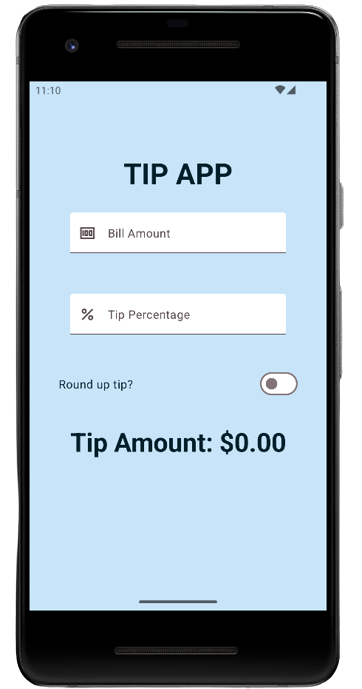
\includegraphics[width=0.8\textwidth, height=8cm, keepaspectratio]{\tipApp}
        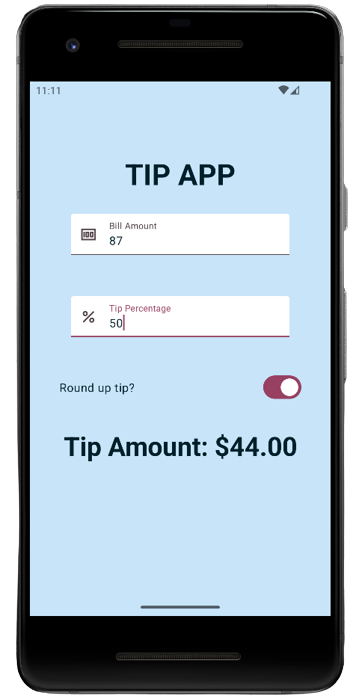
\includegraphics[width=0.8\textwidth, height=8cm, keepaspectratio]{\tipAppAmount}
        \end{center}
        \textbf{\caption{Capturas de Tip-Calculator App}}
    \end{figure}

    \vspace{0.5cm}
    
    \subsection{Aplicacion que permite tirar un dado y mostrar el resultado}
    
    \vspace{0.5cm}
    
    \begin{figure}[h]
        \begin{center}
        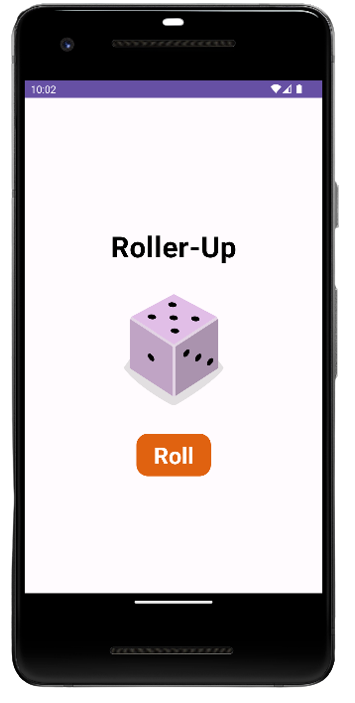
\includegraphics[width=0.8\textwidth, height=8cm, keepaspectratio]{\diceRoller}
        \end{center}
        \textbf{\caption{Capturas de Roller-Up App}}
    \end{figure}

    \vspace{0.5cm}

    \subsection{Aplicacion que exhibe variedad de obras de arte}

    \vspace{0.5cm}

    \begin{figure}[h]
        \begin{center}
        \includegraphics[width=0.8\textwidth, height=8cm, keepaspectratio]{\artSpace}
        \end{center}
        \textbf{\caption{Capturas de Art-Space App}}
    \end{figure}

    \newpage

    \subsection{Aplicacion para realizar tap}

    \vspace{0.5cm}

    \begin{figure}[h]
        \begin{center}
        \includegraphics[width=0.8\textwidth, height=8cm, keepaspectratio]{\onePieceLuffy}
        \includegraphics[width=0.8\textwidth, height=8cm, keepaspectratio]{\onePieceNami}
        
        
        \includegraphics[width=0.8\textwidth, height=8cm, keepaspectratio]{\onePieceZorro}
        \includegraphics[width=0.8\textwidth, height=8cm, keepaspectratio]{\onePieceSanji}
        \end{center}
        \textbf{\caption{Capturas de One piece Tap App}}
    \end{figure}
    
    \vspace{0.5cm}

    \newpage
    
    \section{Opinión del Codelab}
   
    Desde mi perspectiva, este codelab resultó \textbf{notablemente más accesible y claro en comparación con su predecesor}. En diversas instancias, experimenté un progreso fluido sin la necesidad de retroceder en la documentación, lo que ha sido fundamental para consolidar mis bases en el desarrollo de aplicaciones Android con Jetpack Compose.\vspace{0.3cm}
    
    Durante la ejecución de la práctica, logré comprender detalladamente cómo manejar eventos con \textbf{Jetpack Compose}, mejorando mis habilidades en el \textbf{diseño de interfaces y fortaleciendo mis conocimientos} en el desarrollo para Android.\vspace{0.3cm}
    
    Adicionalmente, la sección aborda de manera profunda el tema de \textbf{testing}, aspecto fundamental en el desarrollo de aplicaciones. Aprendí a \textbf{gestionar pruebas automáticas y a manejarme eficientemente en la depuración de la interfaz de Android}. Esta experiencia ha ampliado mi perspectiva sobre las mejores prácticas en testing y depuración, \textbf{elementos esenciales para el desarrollo de aplicaciones robustas y de alta calidad}.

    
\end{document}